\section{Design e \gloss{usabilità} mobile}
Il design dell'applicazione è stato pensato ispirandosi ai principi di material design
e facendo riferimento a diversi scritti di Luke Wroblewski \cite{lukew}.

\subsection{Utilizzo di schede e liste}\label{schede-liste}
Dovendo l'applicazione mostrare soprattutto dati su spazi ristretti come lo schermo
di uno smartphone è stata necessaria una riflessione sui mezzi grafici da usare e
su come trasporre dati mostrati su \fiscoloWeb{} in forma tabellare. \\

Secondo material design:
\begin{itemize}
\item Una \textbf{scheda} è una componente con dati che servono da punto di accesso
ad altri dati. Hanno larghezza fissa ma altezza variabile, sono consigliate qualora
debbano contenere più di tre righe di testo.
\item Una \textbf{lista} è una componente che contiene un insieme di dati omogenei,
o più sottoinsiemi di dati, presentandoli in modo compatto. Ad un elemento di lista
possono essere associate un'azione principale ed un'azione secondaria, si ha accesso
alla prima cliccando su di un'area che comprende la maggior parte della superficie
dell'elemento, si ha accesso alla seconda cliccando sull'estremità destra dell'elemento.
\end{itemize}

Vi sono diverse regole per la composizione grafica di questi elementi, il rispetto
di queste è stato aiutato dall'utilizzo di material ui (cfr. \ref{material-ui}). \\

Sono state utilizzate \textbf{liste} per le seguenti pagine:
\begin{itemize}
\item \textbf{Elenco \gloss{costi} vari}: una volta definite le diverse categorie di costi vari non
ci si aspettano descrizioni particolarmente lunghe, una lista dunque riesce a presentare
i dati salienti (categoria, data, importo) a colpo d'occhio. Qualora venisse inserita
una descrizione più approfondita, cliccare su di un elemento apre una finestra di dialogo
con la descrizione completa.
\item \textbf{Lista progetti}: i progetti devono solamente poter essere scorsi per selezionare
le diverse attività da prendere in carico. Mostrano il proprio nome e una data di scadenza,
se presente, cliccare su un elemento di lista mostra la lista di attività relative.
\item \textbf{Lista attività}: le attività servono solamente per poter essere prese in carico,
mostrano il proprio nome e, qualora fossero già state prese in carico, l'immagine profilo
dell'utente relativo/a. Cliccare su di un elemento di questa lista prende in carico l'attività
relativa.
\item \textbf{Lista promemoria}: in questo caso la lista è divisa in due parti, ovvero i promemoria
"attivi" e quelli già conclusi. Gli elementi di questa lista offrono una azione principale
ed una secondaria, l'azione principale apre una finestra di dialogo che mostra la descrizione
completa del promemoria e offre la possibilità di concluderlo (oppure di riaprirlo qualora
si selezionasse un promemoria già concluso), l'azione secondaria (che si ottiene cliccando
sull'icona a destra dell'elemento) apre una finestra di dialogo che permette di cancellare
il promemoria.
\end{itemize}

Sono state utilizzate delle schede per le seguenti pagine:
\begin{itemize}
\item \textbf{Lista \gloss{relazioni}}: una relazione consiste di una data, una descrizione, un
eventuale indirizzo, una categoria (telefonata, email, incontro) e il nome di un
\gloss{contatto}.
Si è pensato di utilizzare delle schede anche in vista di eventuali sviluppi futuri,
ad esempio qualora venisse fornito un indirizzo potrebbe essere mostrata una mappa.
Allo stato attuale le schede mostrano la categoria di relazione (tramite un'icona),
la data, il nome del contatto e la descrizione.
\end{itemize}

\subsection{Bottoni}\label{bottoni}
Secondo material design:

\begin{itemize}
\item Un bottone deve comunicare chiaramente l'azione ad esso associata, tramite
testo, icone o immagini
\item Un bottone sollevato (\textbf{raised button}) è preferibile quando si vuole
evidenziare un'azione in un ambiente prevalentemente piatto o particolarmente ricco
di altri elementi
\item Un \textbf{floating action button} serve per promuovere una particolare azione,
inoltre può avere una collocazione tale da rendere la funzionalità associata sempre
facilmente raggiungibile all'utente.
\end{itemize}

In \fiscoloMobile{} sono stati utilizzati per alcune azioni dei \textbf{raised button}
mantenuti, per consistenza, uguali a quelli di \fiscoloWeb{}. \\

Ovunque possibile si sono inseriti dei \textbf{floating action button} per evidenziare
le azioni primarie e per renderle sempre disponibili agli utenti, tali bottoni sono
quasi sempre posti nell'angolo in basso a destra della schermata per essere facilmente
raggiungibili col pollice:

\begin{itemize}
\item Nelle pagine che mostrano liste di costi, relazioni, promemoria è presente un
bottone per aggiungere un nuovo costo
\item Nella pagina del timer è presente un bottone per far partire/bloccare il timer
\item Nella pagina contenente la form per inserire un nuovo costo è presente un bottone
per scattare una foto allo scontrino o aggiungerne una dalla galleria del telefono (si è
pensato che questa è l'utilità principale di inserire un costo da mobile)
\end{itemize}

\subsection{Animazioni}\label{material-animation}
Material design sottolinea l'importanza del movimento e delle animazioni per dare un
senso di spazialità e concretezza agli utenti. Nello specifico sono richieste delle
animazioni che siano logicamente correlate con le azioni degli/delle utenti.

\begin{itemize}
\item Gli elementi di un'applicazione devono essere percepiti come tangibili, anche
se separati dall'utente da uno strato di vetro, per far questo devono rispondere agli
input, ad esempio con \textbf{reazioni di superificie} (\textit{\gloss{touch ripple}})
le quali confermano
e riconoscono istantaneamente l'input ricevuto. \textbf{Nb}: tali reazioni devono
partire dal \textit{punto di contatto}. \\
In questo caso Material Ui (cfr. \ref{material-ui}) ha fornito in automatico le animazioni
necessarie, si è quindi riusciti a rispettare i principi di material design.
\item La navigazione tra diverse pagine deve essere accompagnata da
\textbf{transizioni} significative, che aiutino le/gli utenti a concentrare la loro
attenzione nei punti di maggiore importanza. \\
Non si è riusciti a rispettare questo punto in quanto Material Ui non fornisce supporto
alle transizioni e in generale non è stata trovata documentazione di supporto per
React.
\end{itemize}

\subsection[Password e schermata di login]{Password e schermata di login}\label{password}

Lo studio di diversi aspetti di usabilità mobile ha portato a mettere in dubbio un elemento
di sicurezza da sempre dato per scontato: la mascheratura delle password nelle schermate di
login. \\
L'articolo citato in \cite{luke-pass}, oltre ad elencare diversi dati sul rapporto di utenti di diversi servizi
con le password (interessante la citazione di una ricerca del 2006 secondo la quale le quattro
password più usate su MySpace erano \textit{password1}, \textit{abc123}, \textit{myspace1} e
\textit{password}) fa alcune considerazioni interessanti:

\begin{itemize}
\item L'input dalla tastiera di un computer è già prono ad errori, da mobile ancora di più
\item Le tastiere touch degli smartphone danno delle conferme visuali alla pressione di un
carattere (vengono evidenziati seguendo sostanzialmente quanto detto in \ref{material-animation}),
un occhio allenato può quindi leggere il testo inserito anche se questo viene mostrato
mascherato sullo schermo
\item La dimensione ridotta di uno smartphone rende più semplice il celarne lo schermo
da sguardi indiscreti
\end{itemize}

Nonostante queste considerazioni il mascheramento delle password è un pratica comune
alla quale la quasi totalità degli/delle utenti del web e in generale dei sistemi informatici
è abituata.\\

Viene citato un test (\cite{pass-test}) condotto nel 2014 il quale mostra che:

\begin{itemize}
\item La semplice rimozione della maschera dai text field per l'inserzione delle password
causa sorpresa negli/nelle utenti (l'80\% non se lo aspetta) fino ad arrivare al sospetto
(il 60\% riporta una perdita di fiducia nel sito)
\item Togliere la mascheratura di default, offrendo però la possibilità di riattivarla,
viene visto dalla totalità degli/delle utenti come una funzionalità aggiuntiva del sistema.
Vengono colti i vantaggi di usabilità dati dalla possibilità di controllare il testo
inserito come password e i vantaggi di sicurezza di poterlo occultare in caso di necessità.
\end{itemize}

In \fiscoloMobile{} si è dunque scelto di implementare questa funzionalità mostrando di
default la password e permettendo di occultarla con un \gloss{tap} su di un'icona a forma di
occhio
(si perde leggermente in chiarezza rispetto a un pulsante con del testo, ma si è fatto un
compromesso per questioni di design).

\begin{figure}[H]\label{imgLoginPassword}
	\centering
	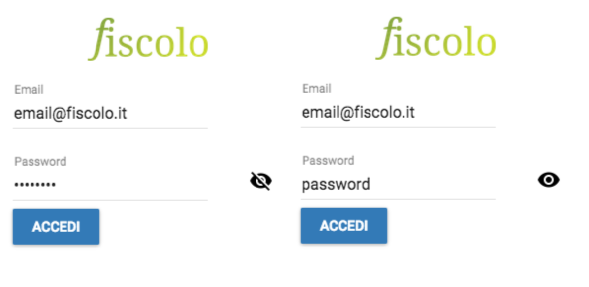
\includegraphics[width=.8\columnwidth]{images/loginPage.png}
	\caption{Schermata di login di \fiscoloMobile}
\end{figure}

\subsection[Menù a tendina]{Menù a tendina}

Nell'articolo citato in \cite{luke-dropdown} vengono sconsigliati i menù a tendina, questo perché:

\begin{itemize}
\item Selezionare un elemento da un menù a tendina richiede in media tre/quattro
tap: apertura, uno o due scroll, selezione
\item Lo scroll è un'operazione imprecisa e può essere frustrante dover scorrere
liste molto lunghe
\end{itemize}

Vengono proposte due alternative:

\begin{itemize}
\item \textbf{Stepper}: si tratta di controlli composti da due pulsanti che permettono
di aumentare e diminuire di un valore fisso una certa quantità
\item \textbf{Radio group}: permettono di selezionare un'opzione da un insieme di
possibilità mutualmente esclusive
\end{itemize}

In \fiscoloMobile{} sono stati sfruttati i \textbf{radio group} per l'aggiunta di nuove
relazioni o di nuovi costi. Per facilitare la selezione non sono stati usati i radio group
di default di Material Ui, i bottoni sono stati invece implementati manualmente sulla falsariga
dei \textit{floating action buttons} di material design, ma differenziati da questi per
colorazione ed altezza dallo sfondo e ombreggiatura.  \\

\begin{figure}[H]\label{imgRadioGroup}
	\centering
	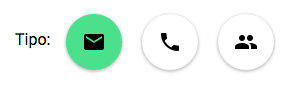
\includegraphics[width=.5\columnwidth]{images/radioGroup.png}
	\caption{Radio group di \fiscoloMobile}
\end{figure}

Per le diverse categorie di costo è stato invece necessario utilizzare un menù a tendina
in quanto queste sono definite dagli utenti e possono quindi aumentare in modo arbitrario.

\subsection{Considerazioni varie}

Seguono alcune considerazioni che non necessitano di una sezione specifica:

\begin{itemize}
\item Buona norma di usabilità è \textit{non presentare liste vuote} ma dei messaggi esplicativi
che comunichino che non ci sono elementi da mostrare. Questo è stato implementato in
\fiscoloMobile{} per le pagine con liste e liste di schede e per le pagine di ricerca.
\item Per la navigazione è stato scelto un menù laterale che appare alla pressione
del pulsante in alto a sinistra sulla barra di navigazione. Tale menù si apre e chiude senza
cambiare pagina aiutando quindi a non disorientare gli/le utenti, inoltre rende facilmente
estendibile l'applicazione con nuove pagine in rilasci successivi.
\item Si è scelto di utilizzare la Home Page per presentare le informazioni relative all'azienda
dell'utente. Questa scelta è stata dovuta principalmente a questioni di tempo: una versione
più complessa ma più utile e interessante avrebbe potuto mostrare dinamicamente le ultime
informazioni rilevanti (nuove attività assegnate, lista di \gloss{promemoria} non conclusi, scadenze
da rispettare) ecc.
\item La ricerca su liste di elementi è stata implementata in modo tale da mostrare dinamicamente
solo gli elementi il cui nome contenga il testo inserito fino a quel momento

\begin{figure}[H]\label{imgSearch}
	\centering
	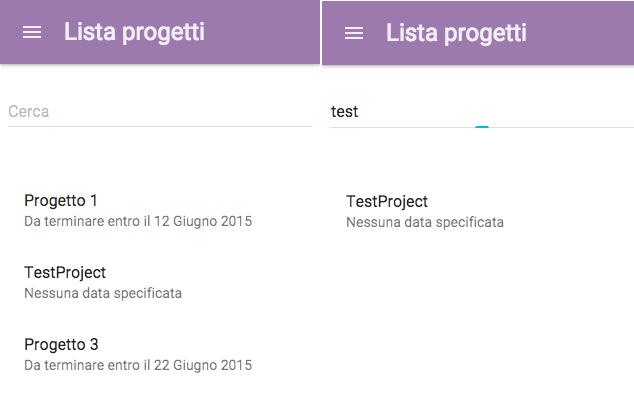
\includegraphics[width=.8\columnwidth]{images/search.png}
	\caption{Esempio di ricerca}
\end{figure}

\end{itemize}
